\documentclass[10pt,a4paper]{article}
\usepackage[utf8]{inputenc}
\usepackage{amsmath}
\usepackage{amsfonts}
\usepackage{amssymb}
\usepackage{graphicx}
\graphicspath{ {../img/} }
\author{Gradey Cullins}
\title{Assignment 2}
\begin{document}
\maketitle

\section*{1}
\section*{2}

Below is the work for solving the LU factorization of A, B, and C and solving for X.\\

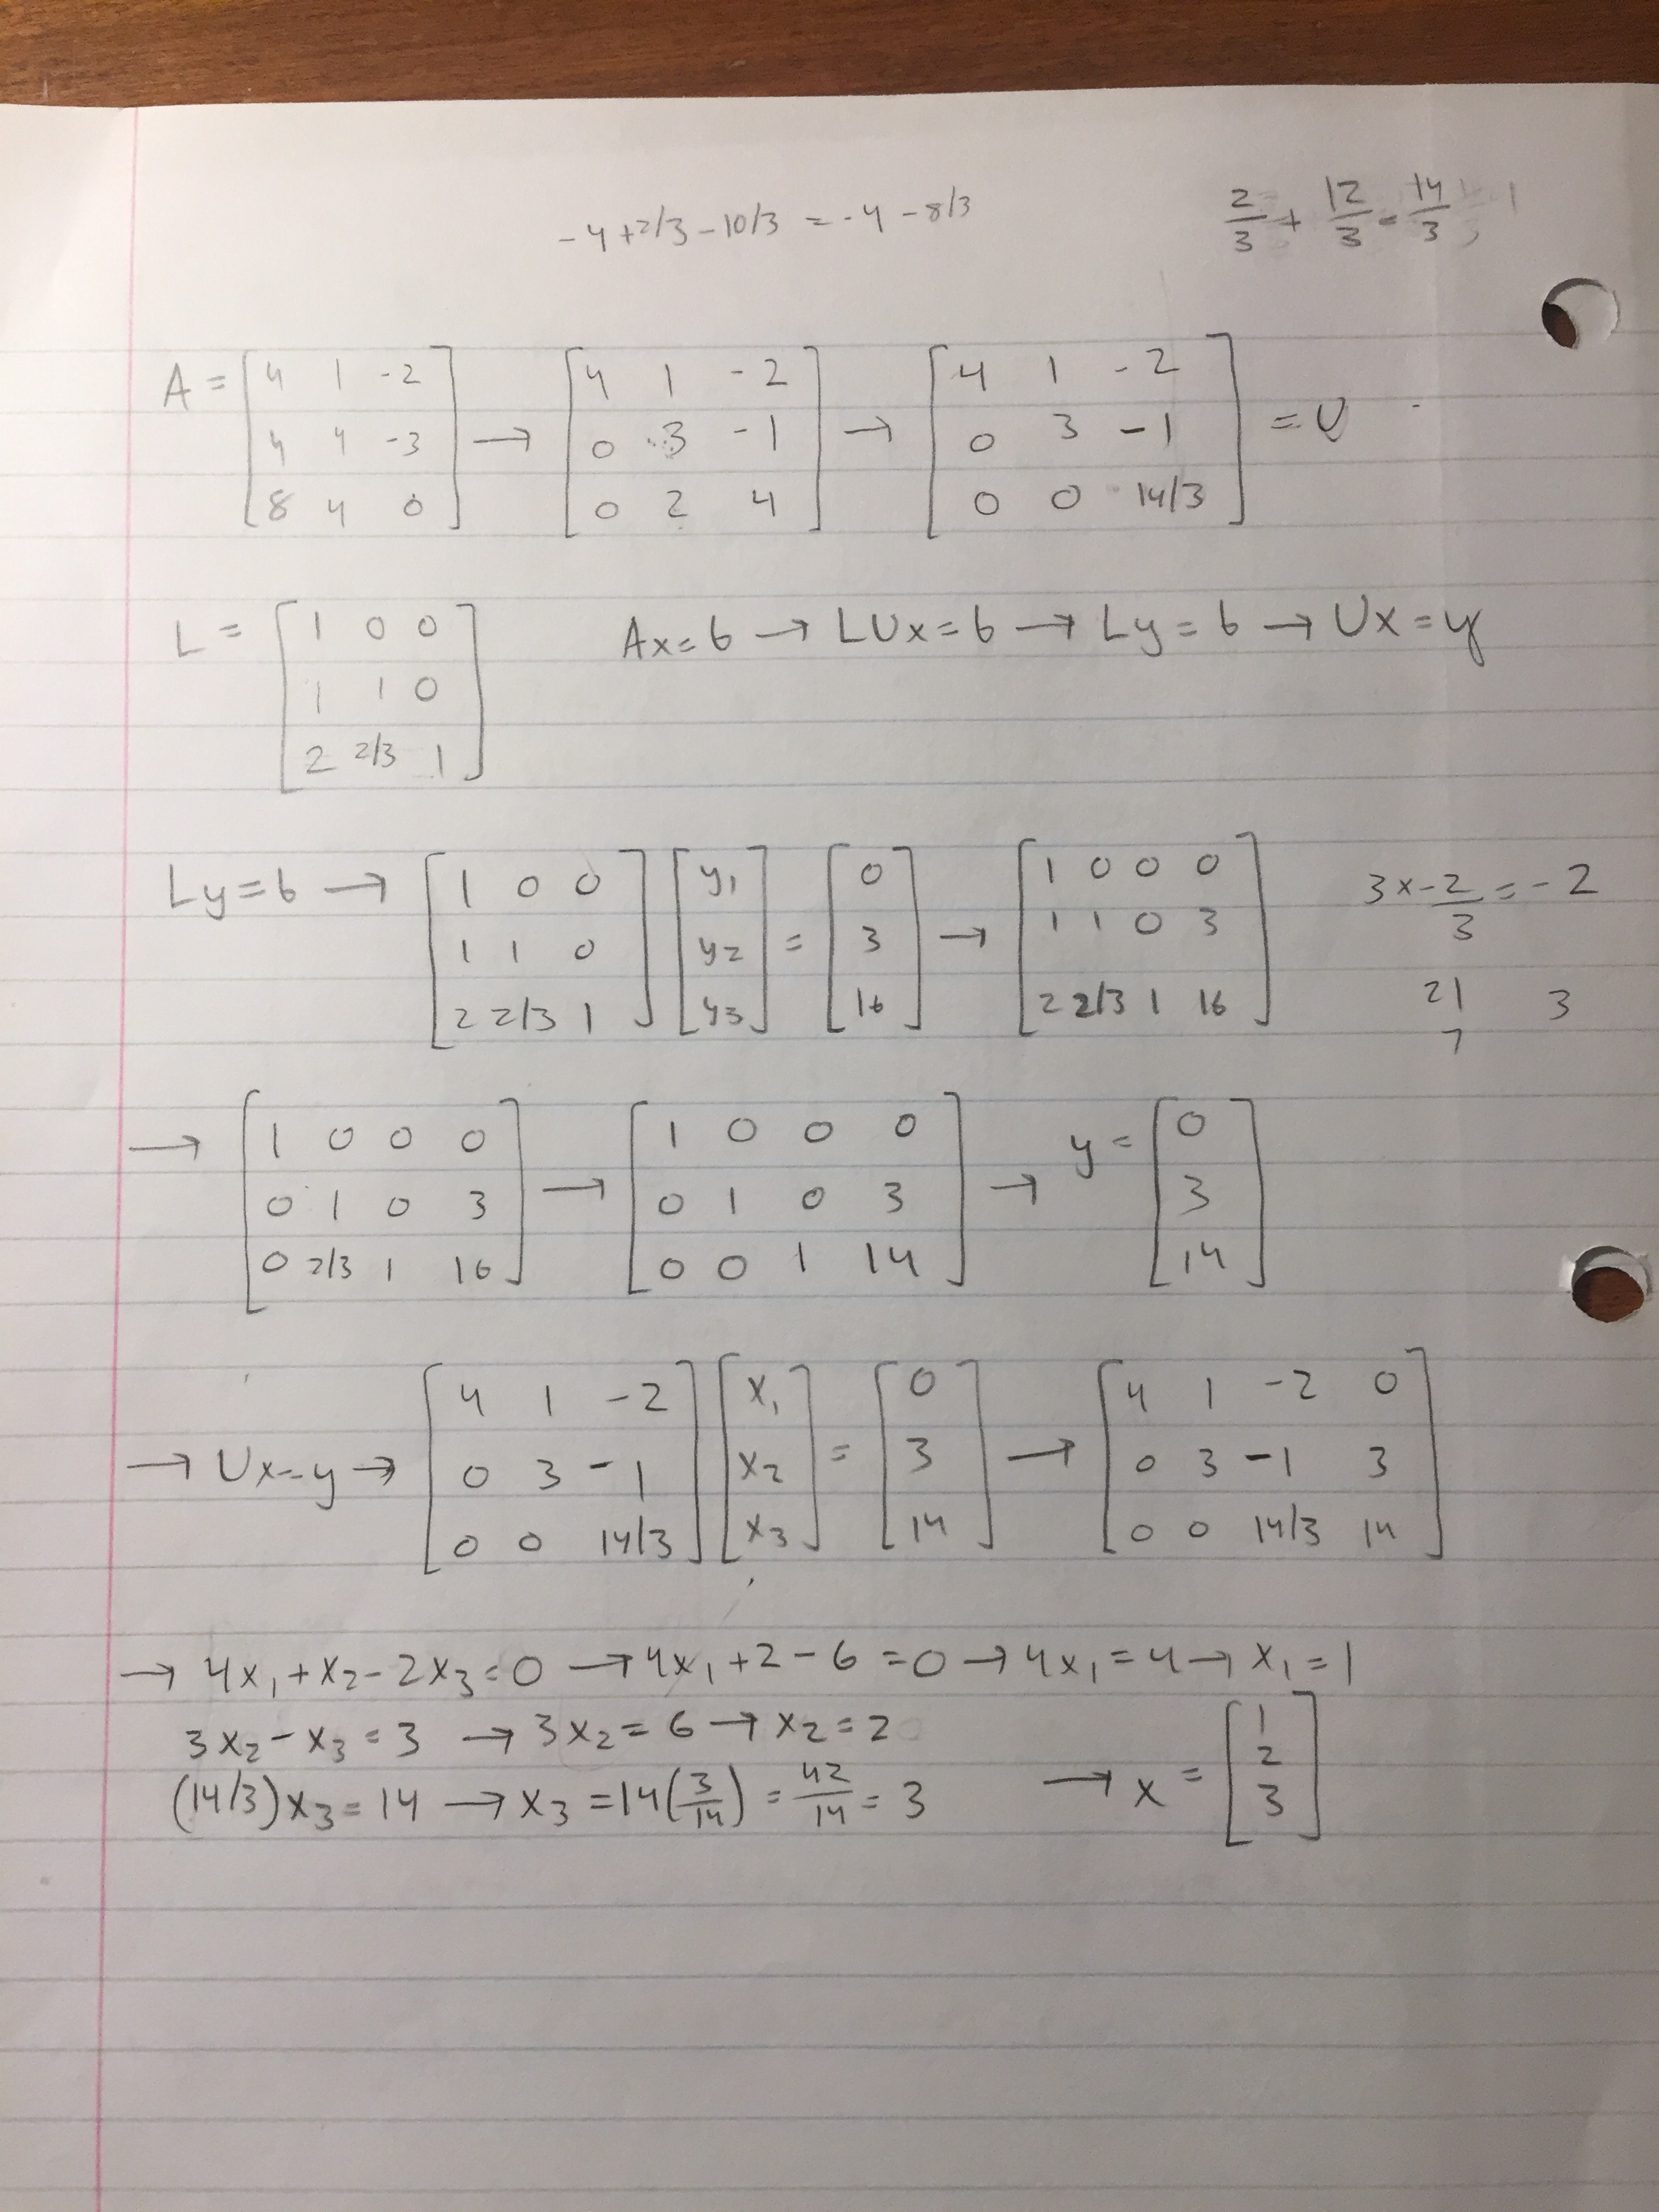
\includegraphics[scale=0.10]{LU_1.JPG} \\
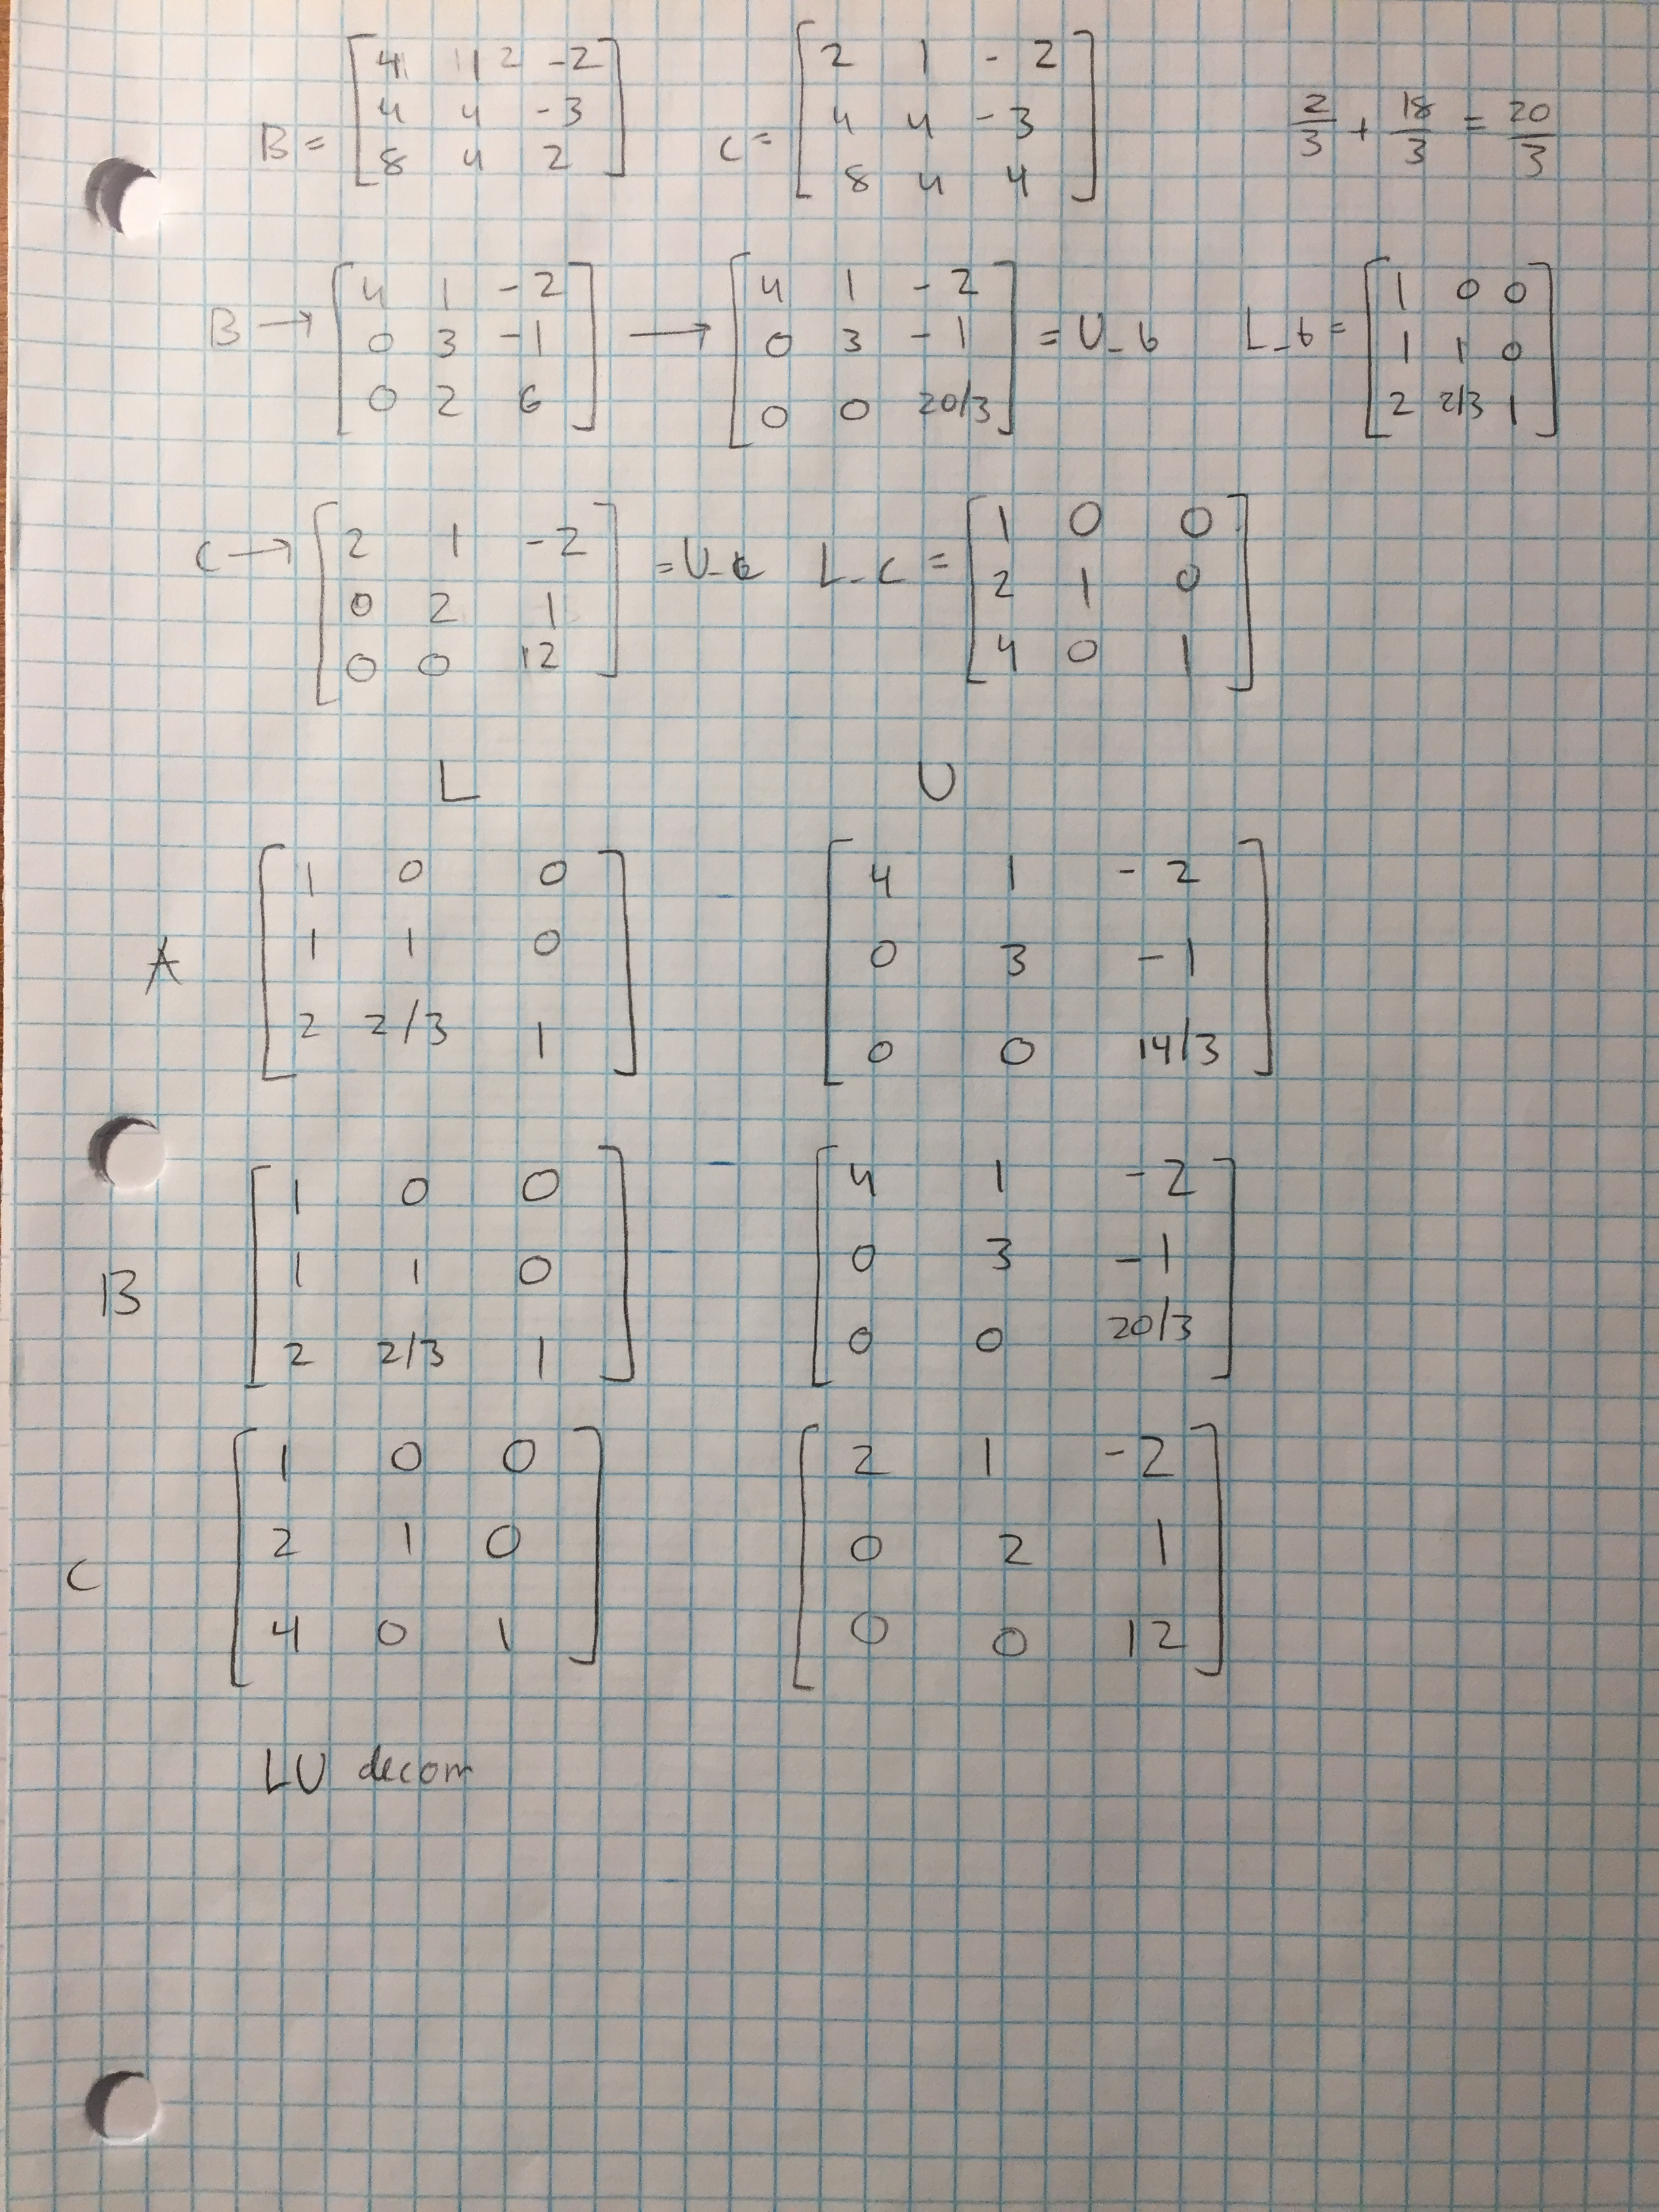
\includegraphics[scale=0.10]{LU_2.JPG} \\

\section*{3}

The LU decompositions of A and B are very similar. The lower matrices $ L_a $ and $ L_b $ are identical, and the upper matrices $ U_a $ and $ U_b $ vary by a singular entry in the (3,3) entry, which corresponds to the differing element from B in the (3,3) entry. This entry is 0 in A, but 2 in B.

The LU decompositions of A and C are somewhat similar, but markedly less similar than the distance between A and B’s LU decompositions. In addition to C containing a mutated entry in the (3,3) entry in comparison to A, it also contains a mutation in the (1,1) entry. My speculation is the the mutation in the (1,1)th entry caused a more drastic variation between A and C’s LU decompositions because the (1,1)th entry is in a pivot position. Pivots tend to be important values, and changing this seems to correspond to a more drastically different decomposition. My hypothesis is supported by two main observations. First, the upper matrix of C or $ U_c $ differs from that of A or $ U_a $ by two entries. Second, the lower matrix of C or $ L_c $ differs from that of A or $ L_a $ by three entries, which is a quite a drastic difference in a 3x3 matrix. 

\section*{4}

Below is a plot of the condition number as a increased for various sizes of N and a. \\

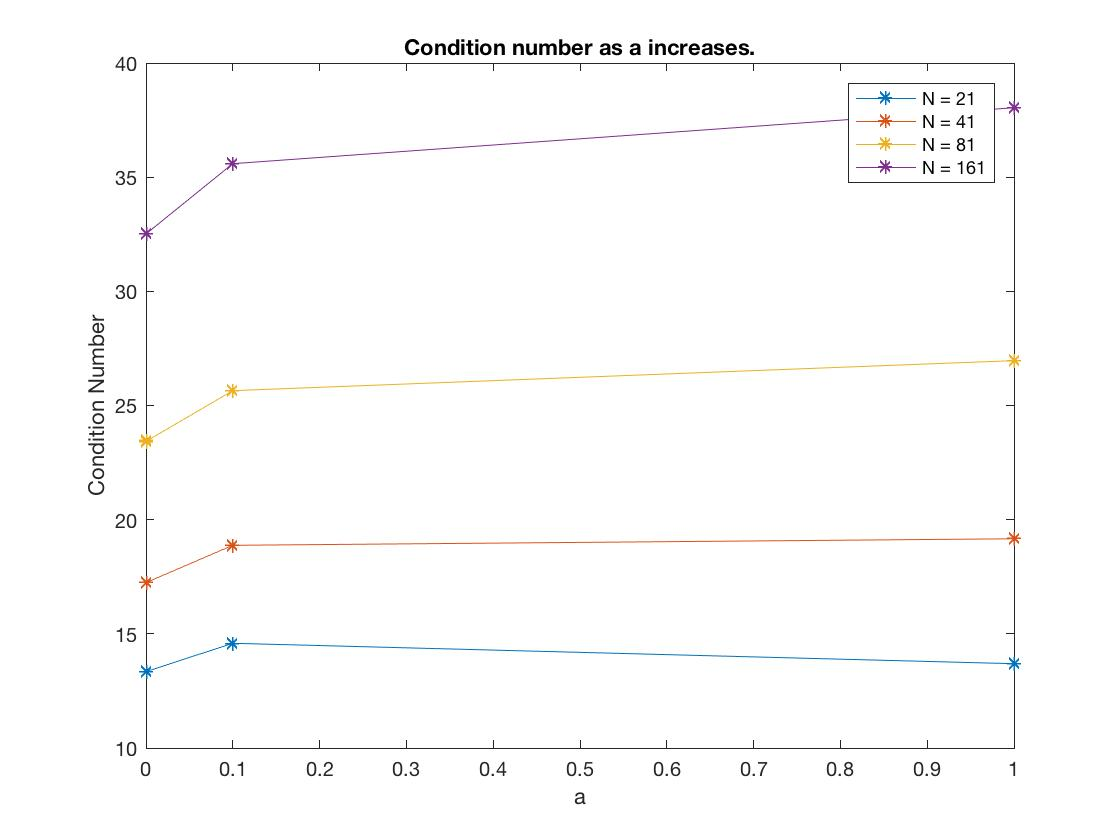
\includegraphics[scale=0.4]{condition_number.jpg} \\

Solution for the equation is below: \\
$ h_1 =  $ [7.0000    6.0000    5.0000] \\
$ h_2 =  $ [8.0000    8.0000    8.0000] \\
$ h_3 =  $ [8.0000    8.0000    8.0000]






\end{document}
